\documentclass[11pt,a4paper]{article}

% ==============================================================================
% PACKAGES & SETUP
% ==============================================================================
\usepackage[utf8]{inputenc}
\usepackage[T1]{fontenc}
\usepackage[margin=1in]{geometry}
\usepackage{amsmath,amssymb,amsfonts}
\usepackage{graphicx}
\usepackage{booktabs}
\usepackage{tabularx}
\usepackage{xcolor}
\usepackage{hyperref}
\usepackage{fancyhdr}
\usepackage{titlesec}
\usepackage{enumitem}
\usepackage{caption}
\usepackage{subcaption}
\usepackage{float}
\usepackage{listings}
\usepackage{microtype}
\usepackage{tcolorbox}

% Colors
\definecolor{primaryblue}{RGB}{26, 35, 126}     % #101657ff
\definecolor{accentblue}{RGB}{63, 81, 181}      % #3f51b5
\definecolor{primaryred}{RGB}{183, 28, 28}      % #b71c1c
\definecolor{accentred}{RGB}{229, 57, 53}       % #e53935
\definecolor{darkgray}{RGB}{33, 33, 33}
\definecolor{lightgray}{RGB}{245, 245, 247}
\definecolor{bordergray}{RGB}{220, 224, 230}
\definecolor{successgreen}{RGB}{46, 125, 50}

\hypersetup{
    colorlinks=true,
    linkcolor=primaryblue,
    citecolor=primaryblue,
    urlcolor=accentblue
}

% Header & Footer
\pagestyle{fancy}
\fancyhf{}
\setlength{\headheight}{14.5pt}
\lhead{\textcolor{darkgray}{\small \textbf{EyeExplore} --- Mid-Term Progress Report}}
\rhead{\textcolor{darkgray}{\small IIIT Bangalore SRIP}}
\cfoot{\thepage}
\renewcommand{\headrulewidth}{0.5pt}

% Section styling
\titleformat{\section}
  {\color{primaryblue}\normalfont\Large\bfseries}
  {\thesection}{1em}{}
\titleformat{\subsection}
  {\color{accentblue}\normalfont\large\bfseries}
  {\thesubsection}{1em}{}
\titleformat{\subsubsection}
  {\color{darkgray}\normalfont\normalsize\bfseries}
  {\thesubsubsection}{1em}{}

% Listings configuration
\lstset{
    backgroundcolor=\color{lightgray},
    basicstyle=\ttfamily\footnotesize,
    breaklines=true,
    captionpos=b,
    commentstyle=\color{gray},
    frame=single,
    rulecolor=\color{bordergray},
    keywordstyle=\color{primaryblue}\bfseries,
    stringstyle=\color{primaryred},
    tabsize=2
}

% Custom boxes
\newtcolorbox{infobox}[2][]{
    colback=lightgray,
    colframe=accentblue,
    fonttitle=\bfseries\color{white},
    title=#2,
    arc=3mm,
    #1
}

\newtcolorbox{alertbox}[2][]{
    colback=lightgray,
    colframe=accentred,
    fonttitle=\bfseries\color{white},
    title=#2,
    arc=3mm,
    #1
}

% ==============================================================================
% DOCUMENT METADATA
% ==============================================================================
\title{
    \vspace{-1.5cm}
    \textbf{\Huge EyeExplore: A Dual-Panel Visual Analytics Workbench for Eye-Tracking, Scanpaths, and Cognitive Attention Dynamics}\\[0.4cm]
    \Large \textbf{Mid-Term Project Progress Report}
}
\author{
    \textbf{SRIP Research Project Team}\\[0.15cm]
    \textit{International Institute of Information Technology Bangalore (IIITB)}\\
    \small Bengaluru, Karnataka, India
}
\date{Academic Session 2026}

% ==============================================================================
% MAIN DOCUMENT
% ==============================================================================
\begin{document}

\maketitle
\thispagestyle{empty}

\begin{abstract}
Eye-tracking provides profound behavioral and cognitive insights into human perception, visual attention, and decision-making processes. However, researchers and UX practitioners frequently face significant hurdles: high software fragmentation, lack of side-by-side comparative capabilities, rigid dataset ingestion pipelines, and absence of temporal metrics distinguishing ambient search from focal inspection. This mid-term report presents the major architectural, algorithmic, and user-experience achievements delivered during the development of \textbf{EyeExplore} (v2.0). 

Key advancements documented in this report include: (1) evolution of the visual layout from a single-panel viewport into a responsive \textbf{dual-panel side-by-side comparative workbench}; (2) integration of \textbf{seven advanced visualization modalities}, including Scanpath Overlays, Scarf Plots, Gaze Co-association Matrices, YOLOv8-powered Object Detection/Semantic AOI generation, Transition Probability Matrices, and real-time Synced Video + K-Timeline playback; (3) deployment of a contextual \textbf{Modal Information System} offering theoretical overviews and interpretation guidelines for every visual tool; and (4) engineering of two entirely new, self-contained dashboard systems: \textbf{My Own Data} (featuring zero-retention in-memory processing, multi-format 3/4-column scanpath ingestion, adaptive multi-modal scene-change keyframing, and coordinate auto-scaling) and the \textbf{K-Coefficient Dataset} (incorporating ambient/focal cognitive modeling across 26 participants, 35,350 fixation events, and a sub-millisecond, requestAnimationFrame-driven HTML5 video-timeline synchronization engine).
\end{abstract}

\vspace{0.3cm}
\tableofcontents
\newpage

% ==============================================================================
% 1. INTRODUCTION & PROJECT MOTIVATION
% ==============================================================================
\section{Introduction and Project Motivation}
\label{sec:introduction}

Eye-tracking technology captures the spatial-temporal coordinates of human gaze, decomposing continuous ocular motor behavior into discrete events: \textit{fixations} (periods where the fovea remains relatively stationary on a visual target to extract optical information) and \textit{saccades} (rapid, ballistic jumps shifting visual gaze from one locus to another). While raw gaze coordinates provide fine-grained spatio-temporal logs, translating these coordinates into actionable cognitive insights requires sophisticated visual analytics platforms.

The \textbf{EyeExplore} project was initiated to build an intuitive, research-grade, web-based visual analytics dashboard that bridges the gap between raw eye-tracking telemetry and cognitive interpretation. The primary objectives established for the mid-term phase were:
\begin{enumerate}[noitemsep,topsep=2pt]
    \item \textbf{Transition to Comparative Analytics:} Replace static, single-viewport rendering with an interactive, side-by-side dual-panel architecture allowing cross-participant, cross-stimulus, and cross-visualization comparisons.
    \item \textbf{Broaden Analytical Encodings:} Implement comprehensive qualitative and quantitative visualizations covering spatial densities, temporal sequences, structural gaze co-associations, automated object boundaries, and state transitions.
    \item \textbf{Self-Guided Analytical Guidance:} Equip the system with contextual explanatory modals to help researchers understand underlying mathematical definitions and practical interpretation strategies.
    \item \textbf{Custom User Ingestion Pipeline (My Own Data):} Develop an end-to-end, zero-retention in-memory ingestion pipeline for arbitrary user images, videos, and heterogeneous CSV/TSV scanpaths.
    \item \textbf{Decompose Cognitive States (K-Coefficient Dashboard):} Operationalize the Eisenberg-Zacks / Unema $K$-coefficient metric to dynamically distinguish exploratory \textit{ambient visual search} from deep \textit{focal inspection} in video viewing.
\end{enumerate}

\begin{figure}[H]
    \centering
    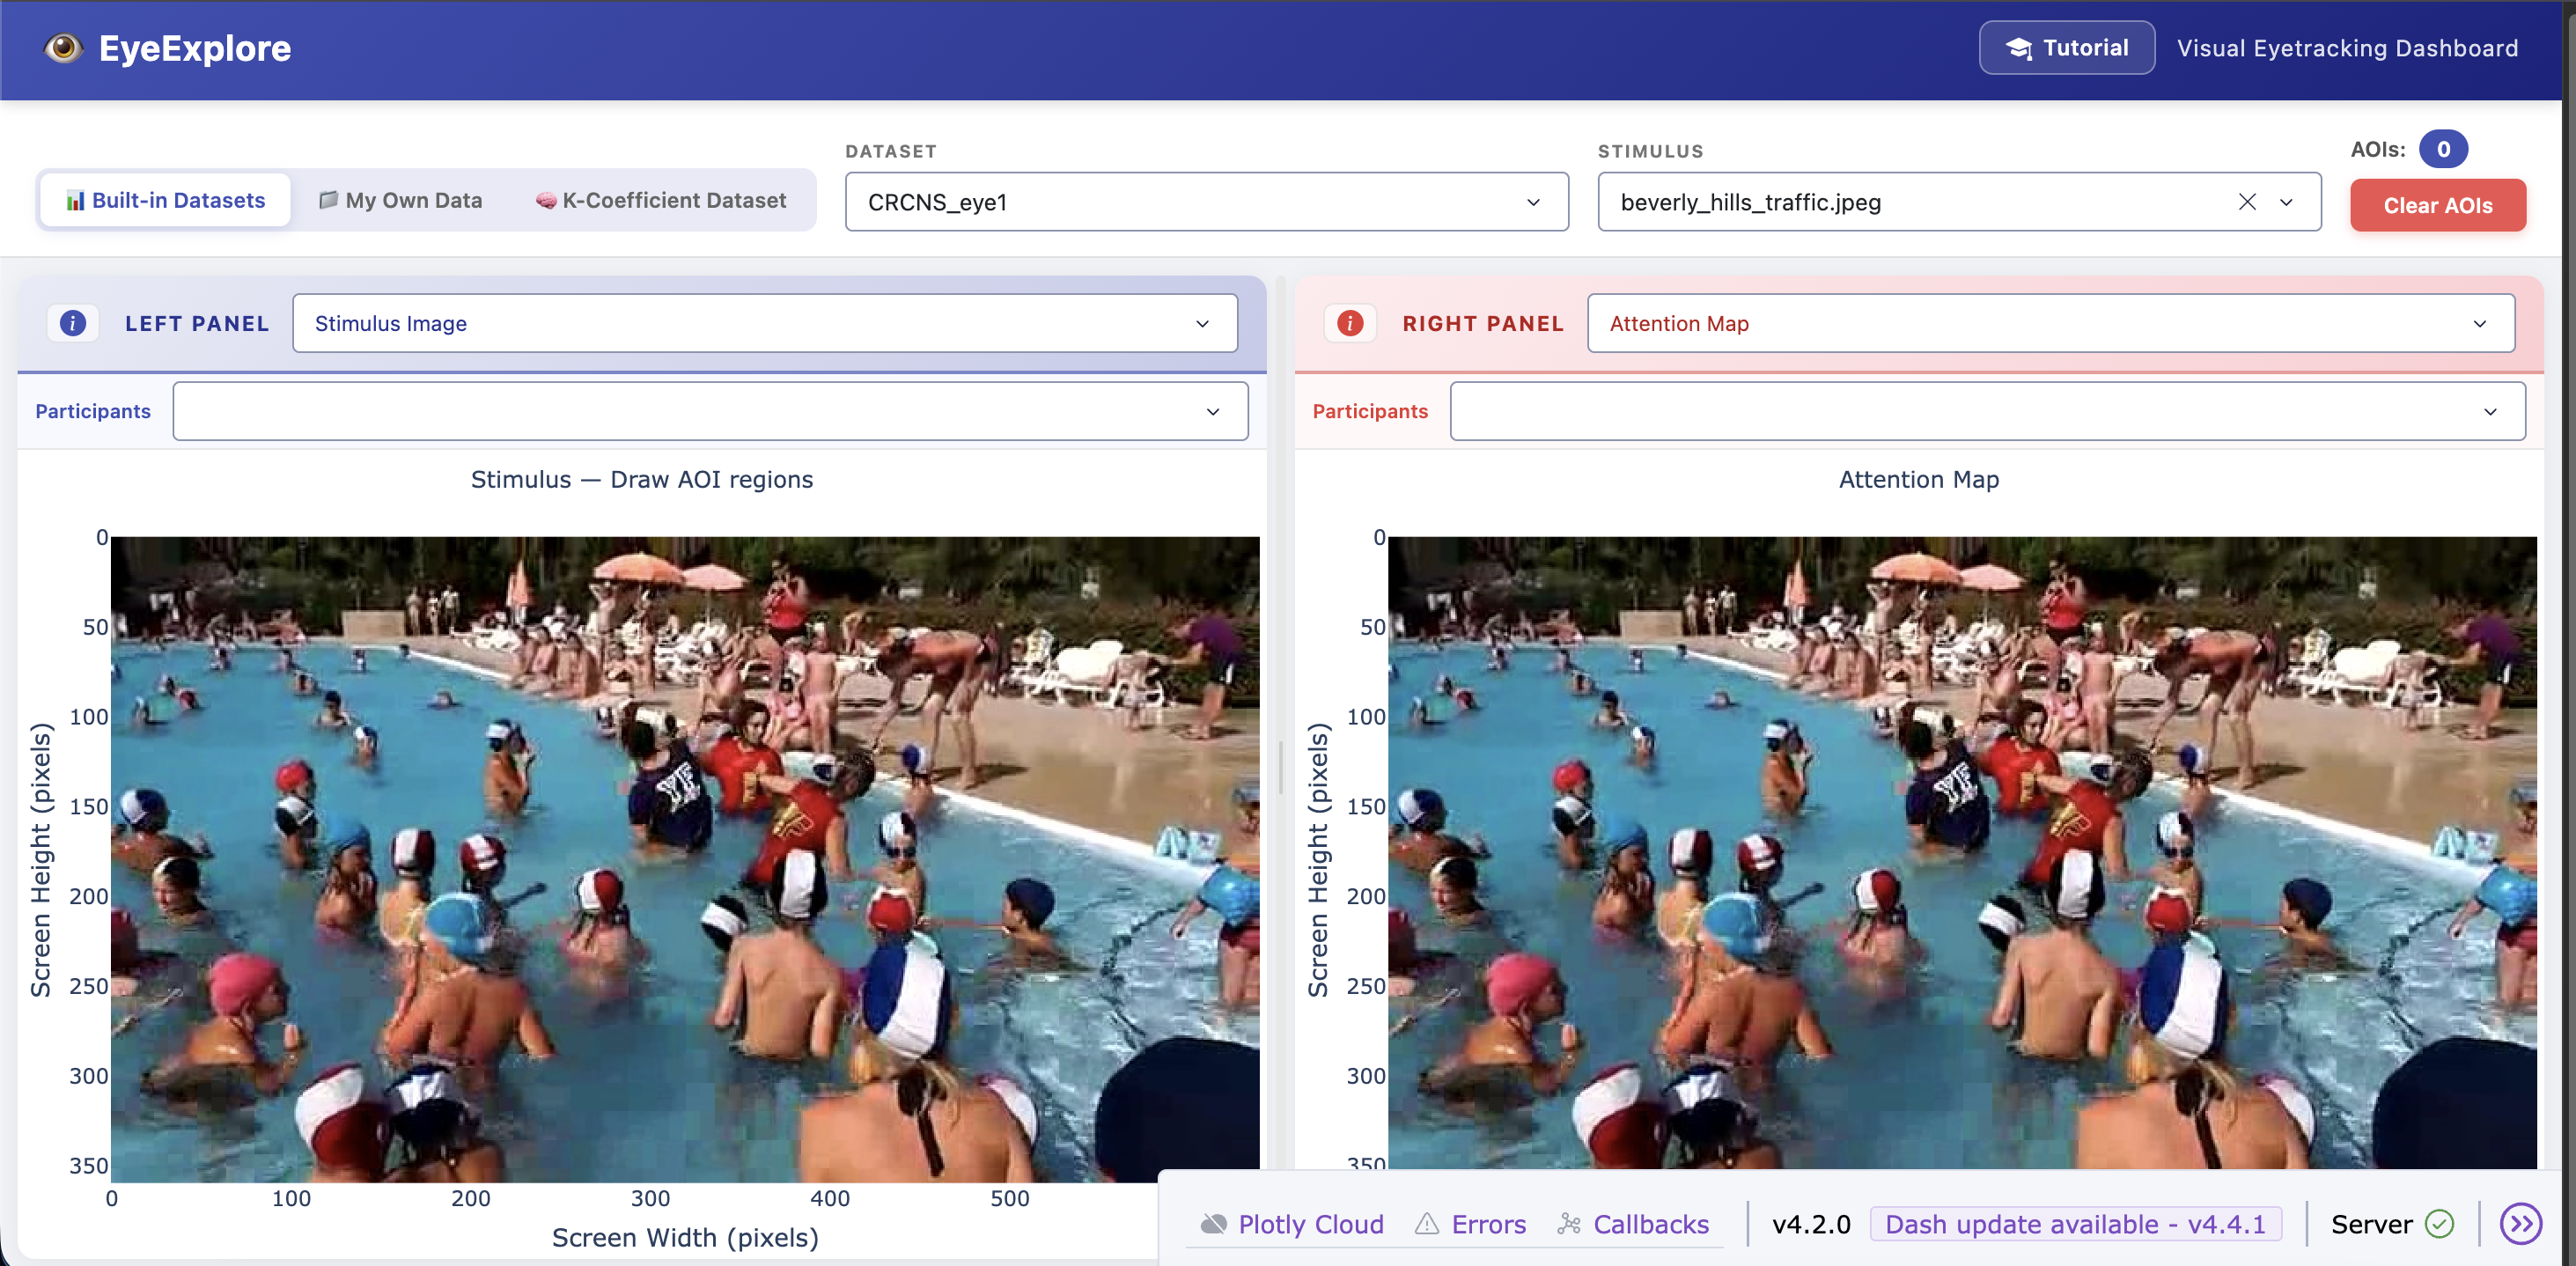
\includegraphics[width=0.98\linewidth]{img1.png}
    \caption{\textbf{EyeExplore Dual-Panel Interface (Built-in Datasets Mode):} Showing the stimulus image with interactive AOI drawing on the Left Panel and the corresponding aggregated Gaussian Attention Map on the Right Panel.}
    \label{fig:builtin_dashboard}
\end{figure}

% ==============================================================================
% 2. ARCHITECTURAL EVOLUTION: DUAL-PANEL COMPARATIVE WORKBENCH
% ==============================================================================
\section{Architectural Evolution: Single- to Dual-Panel Layout}
\label{sec:dual_panel}

\subsection{Design Rationale for Comparative Layout}
In empirical eye-tracking research, absolute visualizations (e.g., viewing an attention heatmap in isolation) rarely provide conclusive evidence. Cognitive psychologists, usability engineers, and radiology researchers must routinely evaluate:
\begin{itemize}[noitemsep,topsep=2pt]
    \item \textbf{Between-Subject Variances:} How novice scanning patterns diverge from expert scanpaths on the exact same stimulus.
    \item \textbf{Spatial vs. Temporal Complementarity:} Simultaneously observing \textit{where} fixations landed on the stimulus (Left Panel: Scanpath Overlay) and \textit{when} or \textit{in what sequence} specific regions were visited (Right Panel: Scarf Plot or AOI Timeline).
    \item \textbf{Continuous Playback vs. Cognitive Classification:} Viewing real-time video gaze dynamics on one side while tracking continuous attention classification ($K$-coefficient) on the other.
\end{itemize}

To satisfy these requirements, the dashboard architecture was fundamentally re-engineered from a single-graph viewport into an independently controlled, synchronized \textbf{Dual-Panel Architecture}.

\subsection{State Management and Decoupled Dispatching}
The user interface is built on Plotly Dash and Dash Bootstrap Components, orchestrated by a central callback mesh in \texttt{app.py}. The dual-panel system maintains independent reactive state containers:
\begin{itemize}[noitemsep,topsep=2pt]
    \item \texttt{left-plot-type} and \texttt{right-plot-type}: Dispatched through distinct dropdown pickers containing the comprehensive suite of 13 visual modalities.
    \item \texttt{left-participants-dropdown} and \texttt{right-participants-dropdown}: Multi-select dropdown elements enabling different sub-cohort selections for each panel.
    \item \texttt{left-graph} and \texttt{right-graph}: Independent Plotly \texttt{dcc.Graph} components housed within flexible CSS flexbox containers with responsive layout boundaries.
\end{itemize}

A visual divider separates the panels, allowing users to resize views dynamically. Figure~\ref{fig:builtin_dashboard} illustrates the dual-panel layout comparing a raw stimulus with an aggregated attention map.

% ==============================================================================
% 3. SUITE OF NEW ADVANCED VISUALIZATIONS
% ==============================================================================
\section{Development of Advanced Visualization Modalities}
\label{sec:visualizations}

Seven major visual analytics modalities were integrated into the dashboard during this project phase:

\subsection{Scanpath Overlay}
\textbf{Purpose:} Qualitative mapping of the complete spatial and sequential progression of gaze for individual participants.
\begin{itemize}[noitemsep,topsep=2pt]
    \item \textbf{Visual Encoding:} Fixations are represented as semi-transparent circular markers whose radii scale monotonically with fixation duration $d_i$:
    \begin{equation}
        r_i = r_{\text{min}} + \alpha \cdot \sqrt{d_i}
    \end{equation}
    where $r_{\text{min}}$ is the base radius and $\alpha$ is a scaling factor.
    \item \textbf{Saccadic Vectors:} Directed line segments with arrowheads connect sequential fixations $(x_i, y_i) \to (x_{i+1}, y_{i+1})$, allowing researchers to immediately inspect visual search directionality, regressions, and scan trajectory efficiency.
\end{itemize}

\subsection{Scarf Plot}
\textbf{Purpose:} A condensed, multi-subject temporal visualization illustrating chronological sequences of Area of Interest (AOI) visits.
\begin{itemize}[noitemsep,topsep=2pt]
    \item \textbf{Visual Encoding:} Each horizontal ribbon corresponds to an individual participant. The horizontal axis represents elapsed experiment time (in milliseconds or seconds).
    \item \textbf{Color Coding:} Contiguous time intervals during which gaze is directed within an AOI are filled with that AOI's unique categorical color. Gaze outside defined AOIs is rendered in neutral gray or transparent white.
    \item \textbf{Utility:} Enables instant visual pattern recognition of whether participant cohorts follow similar reading sequences or skip critical UI components entirely.
\end{itemize}

\subsection{Co-Association Matrix}
\textbf{Purpose:} Quantitative, pairwise similarity evaluation among all participants viewing a common stimulus.
\begin{itemize}[noitemsep,topsep=2pt]
    \item \textbf{Mathematical Formulation:} For a set of $N$ participants, let $S_p$ denote the spatial-temporal fixation sequence of participant $p$. The co-association score $C(p, q) \in [0, 1]$ between participants $p$ and $q$ evaluates the degree of spatial overlap and temporal alignment across discrete time windows:
    \begin{equation}
        C(p, q) = \frac{1}{T} \sum_{t=1}^{T} \exp\left( - \frac{\|\mathbf{x}_p(t) - \mathbf{x}_q(t)\|^2}{2\sigma_{\text{align}}^2} \right)
    \end{equation}
    \item \textbf{Visual Presentation:} Rendered as an $N \times N$ symmetric heatmap with diagonal entries equal to $1.0$. High off-diagonal values denote shared visual attention strategies.
\end{itemize}

\subsection{Automated Object Detection and Semantic AOI Tagging}
\textbf{Purpose:} Eliminates tedious, subjective manual AOI annotation by deploying modern computer vision directly within the visual analytics loop.
\begin{itemize}[noitemsep,topsep=2pt]
    \item \textbf{Architecture:} Incorporates an automated YOLOv8 deep neural network (\texttt{yolov8n.pt}) integrated in \texttt{app.py} and \texttt{semantic\_segmentation.py}.
    \item \textbf{Suppression Algorithm:} Implements an intelligent overlapping box suppression routine combining Intersection over Union (IoU) and Intersection over Minimum Area ($\text{IoMin}$):
    \begin{equation}
        \text{IoU} = \frac{\text{Area}(B_1 \cap B_2)}{\text{Area}(B_1 \cup B_2)}, \quad \text{IoMin} = \frac{\text{Area}(B_1 \cap B_2)}{\min(\text{Area}(B_1), \text{Area}(B_2))}
    \end{equation}
    Boxes exceeding thresholds ($\text{IoU} > 0.3$ or $\text{IoMin} > 0.5$) are filtered in descending order of confidence score.
    \item \textbf{Output:} Generates labeled, shape-accurate bounding boxes around everyday visual elements (e.g., people, cars, screens, text blocks), instantly converting detected entities into formal AOIs.
\end{itemize}

\subsection{Transition Matrix}
\textbf{Purpose:} Probabilistic modeling of visual flow between distinct spatial AOIs.
\begin{itemize}[noitemsep,topsep=2pt]
    \item \textbf{Mathematical Formulation:} Let $M$ be the number of defined AOIs. The transition matrix $\mathbf{P} \in \mathbb{R}^{M \times M}$ stores the conditional transition probability $P_{jk} = P(\text{AOI}_k \mid \text{AOI}_j)$:
    \begin{equation}
        P_{jk} = \frac{n_{j \to k}}{\sum_{m=1}^{M} n_{j \to m}}
    \end{equation}
    where $n_{j \to k}$ is the count of immediate saccadic transitions from $\text{AOI}_j$ to $\text{AOI}_k$.
    \item \textbf{Utility:} Quantifies whether visual hierarchy guides users through the intended sequential path (e.g., Header $\to$ Product Details $\to$ Call to Action).
\end{itemize}

\subsection{K-Coefficient Timeline}
\textbf{Purpose:} Continuous temporal assessment of the participant's cognitive depth of visual processing.
\begin{itemize}[noitemsep,topsep=2pt]
    \item \textbf{Visual Encoding:} Line plot charting the normalized squashed $K$-coefficient ($K_{\text{squashed}} \in [-1, +1]$) against elapsed trial time.
    \item \textbf{Cognitive Shading:} The region above $y = 0$ is shaded soft green, demarcating \textbf{Focal Inspection} (characterized by long fixations following short saccades). The region below $y = 0$ is shaded soft pink, demarcating \textbf{Ambient Exploration} (characterized by short fixations following long saccades).
\end{itemize}

\subsection{Synced Video + K-Timeline}
\textbf{Purpose:} A dynamic, unified multimedia playback environment coupling video stimulus presentation with synchronized cognitive telemetry. Described in detail in Section~\ref{sec:k_dataset}.

\begin{table}[H]
    \centering
    \caption{\textbf{Comprehensive Matrix of Implemented Visualization Modalities}}
    \label{tab:viz_matrix}
    \footnotesize
    \begin{tabularx}{\linewidth}{l X l p{4.2cm}}
        \toprule
        \textbf{Visualization} & \textbf{Primary Analytical Dimension} & \textbf{Input Prerequisite} & \textbf{Cognitive / UX Application} \\
        \midrule
        \textbf{Stimulus Image} & Baseline spatial context & None & Inspection of raw assets; manual AOI drawing. \\
        \textbf{Scanpath Animation} & Dynamic temporal replay & $\ge 1$ Subject & Qualitative review of visual inspection journey. \\
        \textbf{Scanpath Overlay} & Static spatial sequence & 1 Subject & Route efficiency; identification of regressions. \\
        \textbf{Attention Map} & Spatial fixation density & $\ge 1$ Subjects & Hotspot detection; overall visual salience. \\
        \textbf{Scarf Plot} & Multi-subject temporal sequence & AOIs, $\ge 1$ Subject & Cross-subject comparison of AOI visit order. \\
        \textbf{AOI Timeline} & Single-subject AOI presence & AOIs, $\ge 1$ Subject & Dwell time and arrival latency per AOI. \\
        \textbf{3D Scanpath} & Spatio-temporal trajectory ($X, Y, t$) & $\ge 1$ Subject & Disentangling spatial clusters over time. \\
        \textbf{3D Scatter} & Spatio-temporal point cloud & $\ge 1$ Subject & Temporal fixation density in 3D volume. \\
        \textbf{Co-Association Matrix} & Pairwise gaze synchrony & $\ge 2$ Subjects & Measuring consensus across participant cohorts. \\
        \textbf{Object Detection} & Automated semantic bounding & None (AI model) & Rapid, objective AOI creation via YOLOv8. \\
        \textbf{Transition Matrix} & Markovian transition probabilities & AOIs & Evaluation of visual hierarchy flow. \\
        \textbf{Synced Video + K-Timeline} & Multimedia synchronized playback & K-Data, Video & Dynamic tracking of gaze and cognitive state. \\
        \textbf{K-Coefficient Timeline} & Cognitive processing depth over time & K-Data & Discriminating ambient search from focal study. \\
        \bottomrule
    \end{tabularx}
\end{table}

% ==============================================================================
% 4. CONTEXTUAL MODAL INFORMATION SYSTEM
% ==============================================================================
\section{Contextual Modal Information System}
\label{sec:info_modals}

To ensure that both expert researchers and novice practitioners can interpret every visual modality accurately, a comprehensive \textbf{Contextual Information Modal System} was embedded into the dashboard.

\begin{figure}[H]
    \centering
    \begin{minipage}{0.48\textwidth}
        \begin{infobox}{Overview \& Representation}
            \small
            \textbf{Description:} A color-coded overlay aggregating gaze data to show where visual attention was concentrated. Hotter colors (red, yellow) indicate high fixation counts or longer gaze durations.\\
            \textbf{Visual Attributes:} Gaussian-smoothed density surface mapped over the spatial stimulus coordinate frame.
        \end{infobox}
    \end{minipage}
    \hfill
    \begin{minipage}{0.48\textwidth}
        \begin{infobox}[colframe=successgreen]{How to Use \& Interpret}
            \small
            \textbf{Interpretation Guide:} Use heatmaps for quick, at-a-glance insight into interface components attracting primary visual attention.\\
            \textbf{Actionable Insight:} Identify dead zones that fail to attract gaze, and verify whether promotional banners or navigation elements draw expected focal density.
        \end{infobox}
    \end{minipage}
    \caption{Representative content structure rendered by the Contextual Info Modal for the Attention Map.}
    \label{fig:modal_structure}
\end{figure}

\subsection{Engineering Implementation}
In the dashboard header, adjacent to the Left and Right panel dropdowns, circular information triggers (\texttt{left-info-btn} and \texttt{right-info-btn}) were added. When clicked, these buttons trigger Dash Bootstrap Modals (\texttt{left-info-modal} and \texttt{right-info-modal}) containing structured, rich documentation generated dynamically via \texttt{render\_plot\_modal\_content(plot\_type, panel)}.

Each modal delivers a standardized two-tier briefing:
\begin{enumerate}[noitemsep,topsep=2pt]
    \item \textbf{Overview \& Representation:} Explains the underlying mathematical abstraction, data representations, axes, and color schemes.
    \item \textbf{How to Use \& Interpret:} Provides actionable guidelines on how to leverage the visualization for user experience design, cognitive psychology experiments, or clinical diagnostics.
\end{enumerate}

% ==============================================================================
% 5. THE "MY OWN DATA" DASHBOARD
% ==============================================================================
\section{The "My Own Data" Dashboard: End-to-End Custom Ingestion}
\label{sec:my_own_data}

A cornerstone milestone achieved in this phase was the complete engineering of the \textbf{"My Own Data"} dashboard (\texttt{upload\_panel.py} and \texttt{scanpath\_converter.py}). While existing eye-tracking toolkits are often restricted to rigid, pre-packaged datasets, this module empowers researchers to import proprietary stimuli (both static imagery and dynamic video streams) alongside arbitrary scanpath telemetry recorded from commercial eye-trackers.

\begin{figure}[H]
    \centering
    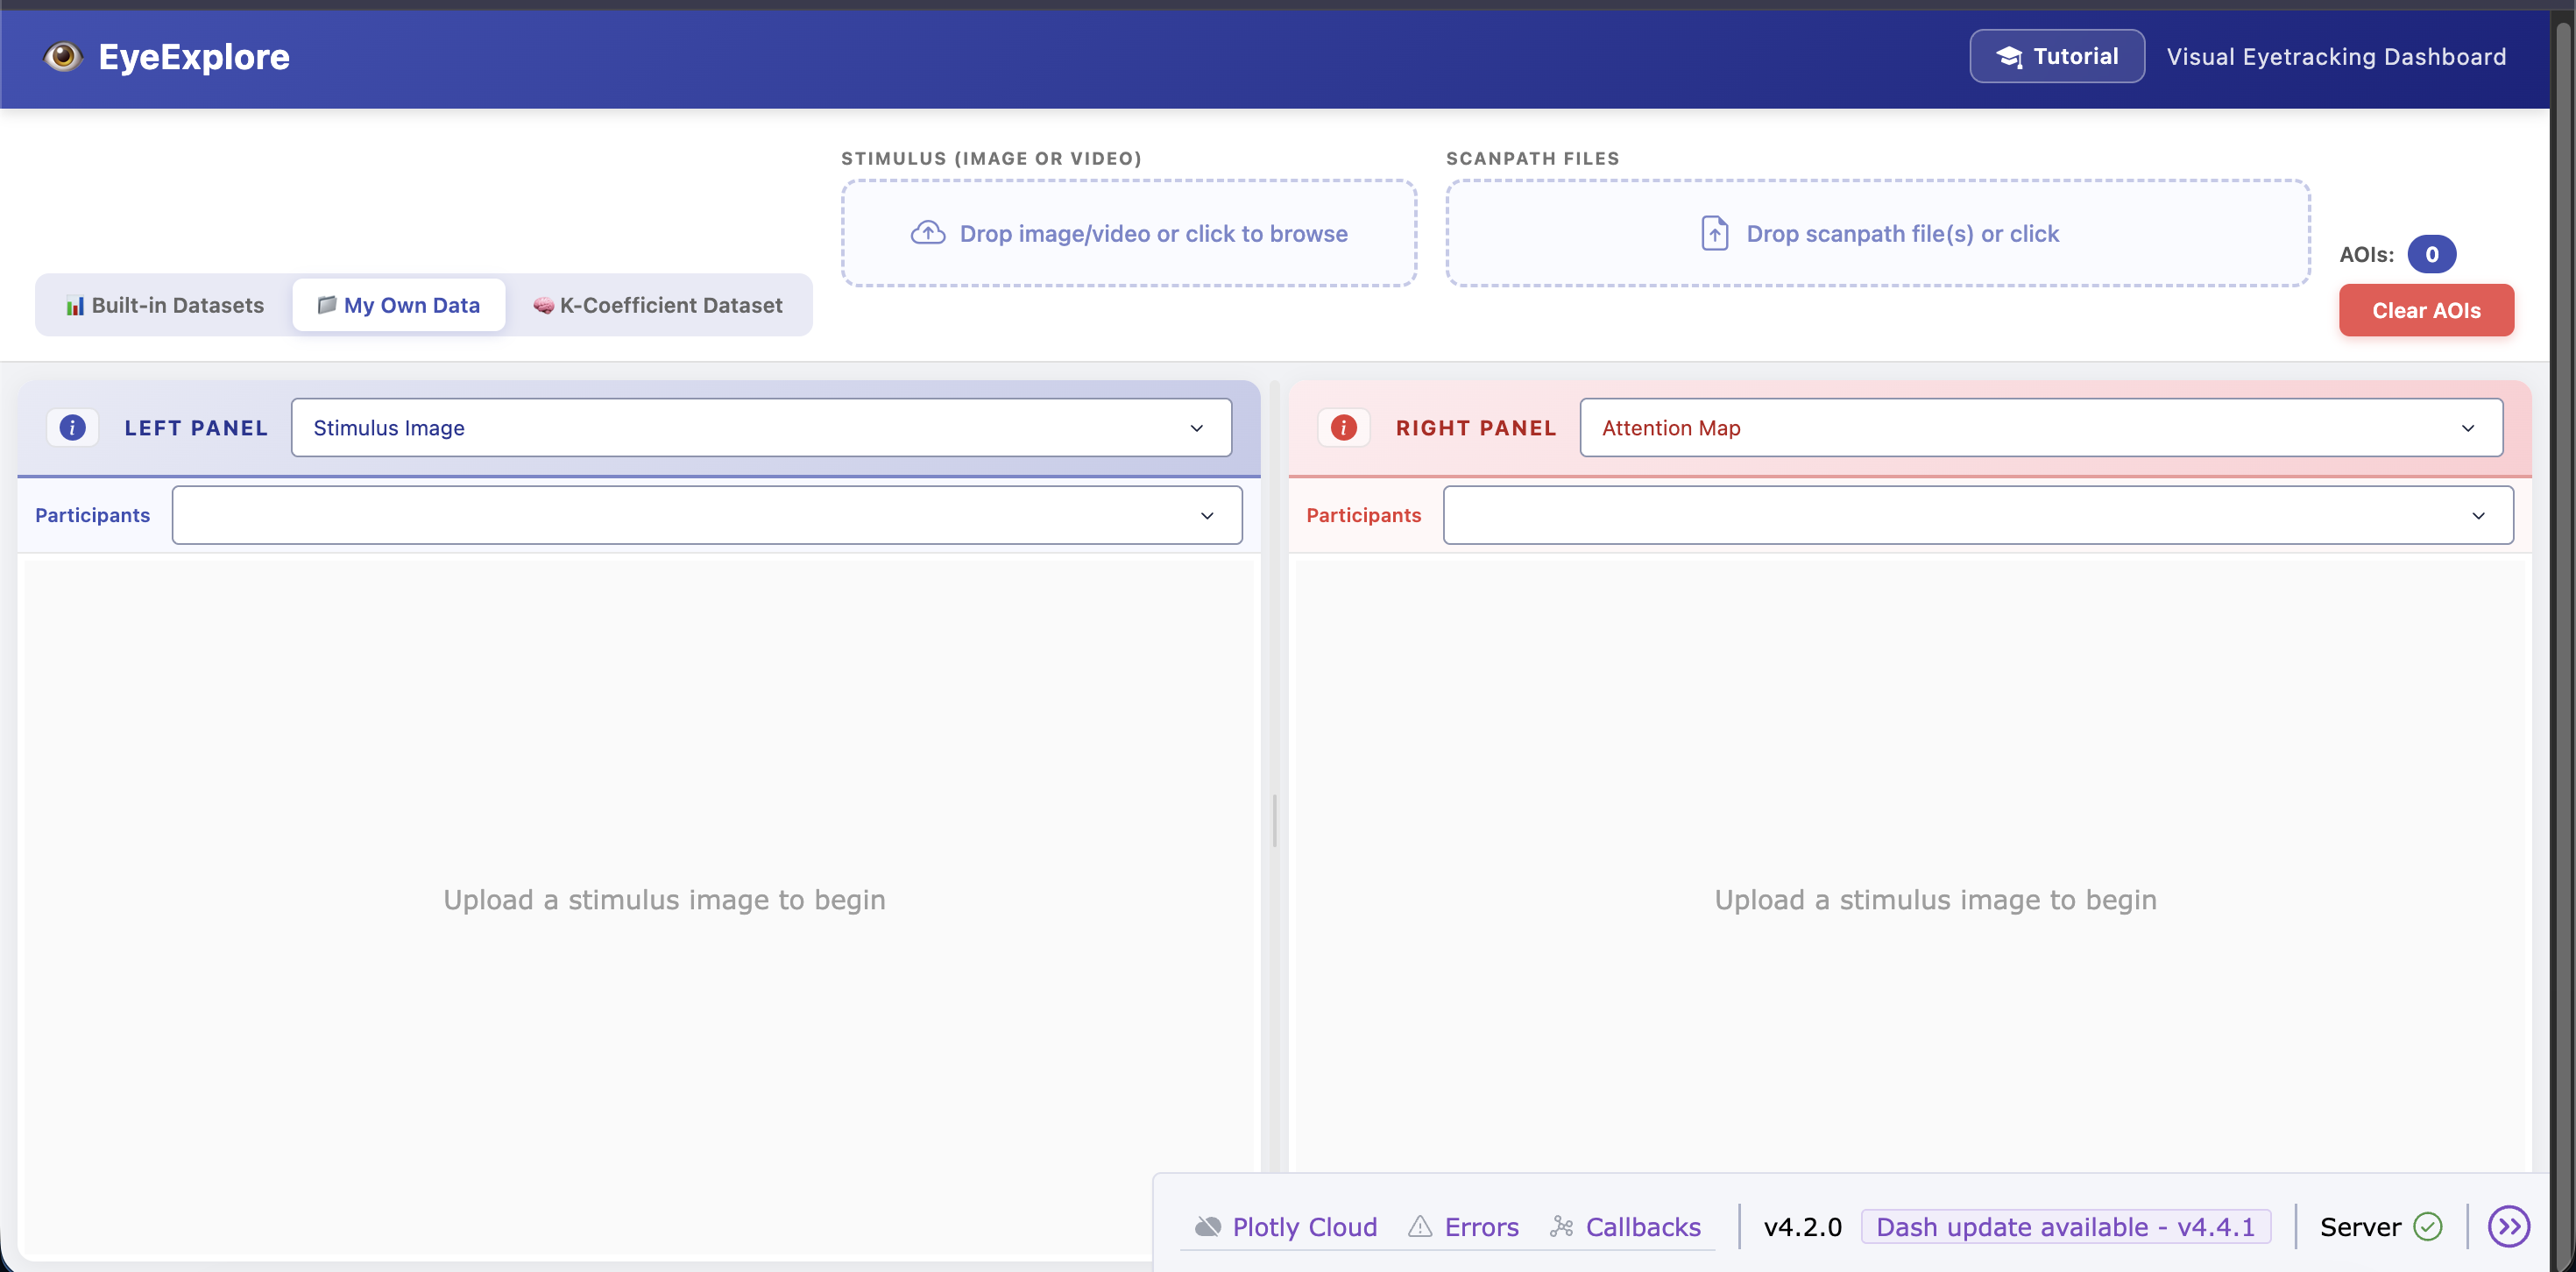
\includegraphics[width=0.98\linewidth]{img2.png}
    \caption{\textbf{"My Own Data" Dashboard Interface:} Highlighting the dual drag-and-drop upload zones for stimulus media (image/video) and scanpath data files, with dual-panel empty states ready for data rendering.}
    \label{fig:my_own_data}
\end{figure}

\subsection{Zero-Retention In-Memory Processing Architecture}
Data privacy is paramount in eye-tracking, where raw ocular telemetry constitutes sensitive biometric data. To ensure full compliance with modern institutional data governance and user privacy mandates, a strict \textbf{zero-retention, in-memory processing architecture} was enforced across the ingestion pipeline:
\begin{itemize}[noitemsep,topsep=2pt]
    \item \textbf{No Disk Persistence:} Uploaded stimuli (images or video files), parsed scanpaths, and extracted keyframe imagery are never written to the server's persistent disk, filesystem cache, or database.
    \item \textbf{Transient Byte Streaming:} Inbound files received through Dash \texttt{dcc.Upload} components are decoded from base64 strings directly into volatile RAM byte buffers (\texttt{io.BytesIO}).
    \item \textbf{Session Destruction on Refresh:} All application state is stored in client-side and memory-bound stores (\texttt{custom-image-store}, \texttt{custom-scanpaths-store}, and \texttt{custom-keyframes-store}). The moment the browser session is terminated or reloaded, all in-memory buffers are instantly destroyed and garbage-collected.
    \item \textbf{Sanitization Barrier:} Filenames are cleansed using a custom \texttt{secure\_filename()} routine that removes path traversal characters (\texttt{..}), slashes, shell operators, and HTML tags, mitigating cross-site scripting (XSS) and arbitrary filesystem exploration risks.
\end{itemize}

\subsection{Multi-Modal Stimulus Media Ingestion}
The stimulus upload pipeline accommodates two distinct visual paradigms:
\begin{enumerate}
    \item \textbf{Static Visual Stimuli:} Supports \texttt{.png}, \texttt{.jpg}, \texttt{.jpeg}, \texttt{.bmp}, and \texttt{.webp} containers (capped at $10\,\text{MB}$). PIL decodes the byte stream, extracts resolution parameters $(W_{\text{stim}}, H_{\text{stim}})$, and generates a thumbnail chip indicating file dimensions and format.
    \item \textbf{Dynamic Video Stimuli:} Supports modern video formats including \texttt{.mp4}, \texttt{.avi}, \texttt{.mov}, \texttt{.webm}, and \texttt{.mkv} (capped at $50\,\text{MB}$). As video decoding requires random-access frame seeking that is computationally prohibitive over raw base64 streams, video bytes are staged in a transient, secured tempfile descriptor (\texttt{tempfile.mkstemp}) that is immediately unlinked upon OpenCV extraction. A dynamic \texttt{dcc.Loading} indicator provides real-time feedback during processing.
\end{enumerate}

\subsection{Adaptive Multi-Modal Scene-Change Keyframe Extraction Algorithm}
Eye-tracking over dynamic video stimuli presents a fundamental visualization paradox: static visual analytics (such as Scanpath Overlays, Gaussian Attention Heatmaps, and YOLO Object Detections) require a fixed spatial canvas. Plotting gaze over a moving video without temporal slicing results in incoherent, visually entangled point clouds.

To resolve this, an \textbf{adaptive multi-modal keyframe extraction algorithm} was developed in \texttt{scanpath\_converter.py}. Rather than sampling at arbitrary fixed intervals (which produces redundant frames during static scenes and misses fast cuts), the algorithm dynamically detects visual scene boundaries using a two-pass computer vision pipeline:

\subsubsection{Pass 1: Subsampled Multi-Modal Feature Extraction}
Frames are sampled at approximately 10 frames per second to ensure real-time responsiveness ($\text{step} = \max(1, \lfloor \text{FPS} / 10 \rfloor)$). For each sampled frame index $i$, two complementary visual feature descriptors are calculated:
\begin{itemize}[noitemsep,topsep=2pt]
    \item \textbf{2D Normalized Color Histogram ($H_i$):} The frame is converted to the HSV color space to decouple chromaticity from illumination. A 2D joint histogram over Hue ($50$ bins, $[0, 180]$) and Saturation ($60$ bins, $[0, 256]$) is computed and min-max normalized to $[0, 1]$.
    \item \textbf{Downsampled Grayscale Structural Frame ($I_{i, \text{small}}$):} The frame is converted to single-channel luminance and resized to a standardized thumbnail ($160 \times 120$ pixels).
\end{itemize}

\subsubsection{Pass 2: Combined Dissimilarity Metric and Adaptive Thresholding}
For consecutive sampled frames $(i-1)$ and $i$, a combined dissimilarity score $S_i \in [0, 1]$ is calculated by fusing chromatic and structural variations with equal weight:
\begin{equation}
    S_i = 0.5 \cdot \Big(1 - \text{corr}(H_{i-1}, H_i)\Big) + 0.5 \cdot \left( \frac{1}{255 \cdot 160 \cdot 120} \sum_{x=1}^{160}\sum_{y=1}^{120} |I_{i-1, \text{small}}(x,y) - I_{i, \text{small}}(x,y)| \right)
\end{equation}
where $\text{corr}(H_{i-1}, H_i)$ represents the Pearson correlation coefficient between histograms.

To ensure robust performance across both high-contrast fast-paced videos and subtle continuous transitions, the algorithm uses an empirical statistical threshold $\tau$:
\begin{equation}
    \tau = \max\Big(0.015, \, \mu_S + 0.15 \cdot \sigma_S\Big)
\end{equation}
where $\mu_S$ and $\sigma_S$ are the mean and standard deviation of $S_i$ across the entire clip. Frames where $S_i \ge \tau$ are selected as keyframe candidates. The first frame ($t = 0.0\,\text{s}$) and the terminal frame ($t = t_{\text{end}}$) are unconditionally included. Candidates are ranked by dissimilarity, capped at $\max(2, \lfloor 5 \times T_{\text{duration}}\rfloor)$ frames, and sorted chronologically.

\subsection{Temporal Keyframe Windowing for Static Visual Analytics}
Each extracted keyframe is indexed with an active temporal window $[\text{Time}_{\text{start}}, \text{Time}_{\text{end}}]$ defining the scene boundaries it represents. When the researcher selects a specific keyframe from the "Key Frames" dropdown (e.g., \textit{"Frame 10 --- 14.5s"}):
\begin{itemize}[noitemsep,topsep=2pt]
    \item The stimulus canvas displays that specific keyframe image.
    \item In static visualization modes (Scanpath Overlay, Attention Map, Object Detection), \texttt{\_get\_custom\_scanpath\_dfs()} filters the participant's scanpath to only fixations satisfying:
    \begin{equation}
        \text{TIME\_FROM} \ge \text{Time}_{\text{start}} \quad \text{and} \quad \text{TIME\_TO} \le \text{Time}_{\text{end}}
    \end{equation}
    \item This enables precise, scene-by-scene cognitive evaluation without visual clutter from preceding or subsequent scenes.
\end{itemize}

\subsection{Dynamic Synchronized Video Playback in "My Own Data"}
Beyond static keyframe analysis, the "My Own Data" dashboard provides a complete \textbf{dynamic synchronized video playback environment}:
\begin{itemize}
    \item \textbf{In-Memory HTML5 Video Delivery:} When a video is uploaded and the user selects the \textbf{"Synced Video + K-Timeline"} visualization on the Left Panel, the graph is swapped for a native HTML5 \texttt{<video>} element (\texttt{\#k-video-player}) fed directly by a base64 data URI (\texttt{data:video/mp4;base64,...}).
    \item \textbf{Client-Side Gaze Tracking Bridge:} The raw scanpath data is serialized into JSON and placed in the hidden bridge container (\texttt{\#k-fixation-data}). The vanilla JavaScript engine (\texttt{assets/k\_sync.js}) automatically connects to the player.
    \item \textbf{Real-Time Fixation Dot Overlay:} During video playback (play, pause, scrub, fast-forward), the animated fixation marker (\texttt{\#k-fixation-dot}) tracks the participant's eye movements directly over the playing video at 60 FPS.
    \item \textbf{Responsive Letterbox Projection:} Because custom videos possess diverse aspect ratios ($16:9$, $4:3$, vertical mobile $9:16$) rendered via CSS \texttt{object-fit: contain}, the synchronization script computes horizontal and vertical pillarbox offsets dynamically, guaranteeing that the gaze dot accurately aligns with video coordinates regardless of screen resizing.
    \item \textbf{Trailing Gaze History:} A sequence of decaying trail nodes follows the primary marker, providing immediate visual feedback on scan velocity and directionality over the video.
\end{itemize}

\subsection{Decoupling K-Timeline from Keyframe Filtering (The Full-Range Fix)}
A critical architectural challenge arose when combining keyframe extraction with temporal cognitive analytics. Initially, when \texttt{custom\_image\_store} was passed to the scanpath slicing function \texttt{\_get\_custom\_scanpath\_dfs()}, it filtered gaze events to the selected keyframe's window (e.g., $0.0\,\text{s}$ to $2.1\,\text{s}$). Consequently:
\begin{itemize}[noitemsep,topsep=2pt]
    \item The K-Coefficient Timeline was truncated to that single keyframe window, hiding the rest of the multi-minute recording.
    \item Video playback beyond the first keyframe resulted in the scrubber line disappearing from the chart.
\end{itemize}

To solve this, the data-fetching pipeline in \texttt{app.py} was refactored:
\begin{itemize}[noitemsep,topsep=2pt]
    \item In \texttt{update\_left\_graph}, \texttt{update\_right\_graph}, and \texttt{populate\_fixation\_data}, calls for K-related visualizations (\texttt{k\_video}, \texttt{k\_timeline}) explicitly pass \texttt{custom\_image\_store=None}.
    \item Passing \texttt{None} bypasses the keyframe temporal filter, supplying the full multi-minute scanpath DataFrame.
    \item As a result, the K-Coefficient Timeline renders the complete experiment duration ($0 \to T_{\text{duration}}$), and the red scrubber line seamlessly tracks the video across all keyframes and scene cuts.
\end{itemize}

\subsection{Scanpath Standardization and Column Mapping Engine}
Scanpath files exported from diverse eye-tracking hardware exhibit substantial structural variability. The ingestion engine in \texttt{scanpath\_converter.py} standardizes arbitrary tabular data:
\begin{itemize}[noitemsep,topsep=2pt]
    \item \textbf{Delimiter Sniffing:} Automatically detects comma, tab, or whitespace separators without manual configuration.
    \item \textbf{Format A (Explicit 4-Column):} Ingests $[X, Y, \text{Start Time}, \text{End Time}]$ with direct passthrough renaming to $[\text{X}, \text{Y}, \text{TIME\_FROM}, \text{TIME\_TO}]$.
    \item \textbf{Format B (Cumulative 3-Column):} Ingests $[X, Y, T]$, where $T_i$ represents cumulative elapsed time at fixation termination. The engine reconstructs discrete event intervals via:
    \begin{equation}
        \text{TIME\_FROM}_0 = 0, \quad \text{TIME\_FROM}_i = \text{TIME\_TO}_{i-1} \quad (i \ge 1), \quad \text{TIME\_TO}_i = T_i
    \end{equation}
    \item \textbf{Interactive Column Mapper:} Renders dynamic dropdown pickers for each detected column. A validation barrier blocks progression if required meanings are omitted or duplicated. A 5-row preview table is rendered for researcher confirmation before commitment.
    \item \textbf{In-Memory AOI Tagging (\texttt{assign\_aoi}):} Evaluates geometric containment of gaze points within drawn rectangular or polygonal AOIs directly on in-memory DataFrames, enabling Scarf Plots and Transition Matrices without external library dependencies.
\end{itemize}

\subsection{Percentage vs. Pixel Coordinate Auto-Scaling}
Many modern eye-trackers record gaze coordinates normalized as percentages ($X, Y \in [0, 100]$) rather than raw display pixels. When overlaid on high-resolution video (e.g., $1920 \times 1080$), these points collapsed into a minuscule $100 \times 100$ pixel square in the upper-left corner.

An automated auto-scaling engine was embedded into \texttt{\_get\_custom\_scanpath\_dfs()}:
\begin{equation}
    \text{If } \max(X) \le 100.01 \text{ and } \max(Y) \le 100.01 \text{ and } W_{\text{stim}} > 200: \quad X \gets X \cdot \frac{W_{\text{stim}}}{100}, \quad Y \gets Y \cdot \frac{H_{\text{stim}}}{100}
\end{equation}
Conversely, when populating the bridge container (\texttt{populate\_fixation\_data}) for the HTML5 overlay, coordinates are converted back into normalized percentages ($x_{\text{pct}} = (X / W_{\text{stim}}) \times 100$) so that CSS percentage positioning functions accurately across all browser viewport dimensions.

% ==============================================================================
% 6. THE "K-COEFFICIENT DATASET" DASHBOARD & GAZE DYNAMICS
% ==============================================================================
\section{The "K-Coefficient Dataset" Dashboard and Gaze Dynamics}
\label{sec:k_dataset}

The third major dashboard tab is dedicated to the \textbf{K-Coefficient Dataset}, operationalizing cognitive attention dynamics for eye-tracking over video stimuli.

\begin{figure}[H]
    \centering
    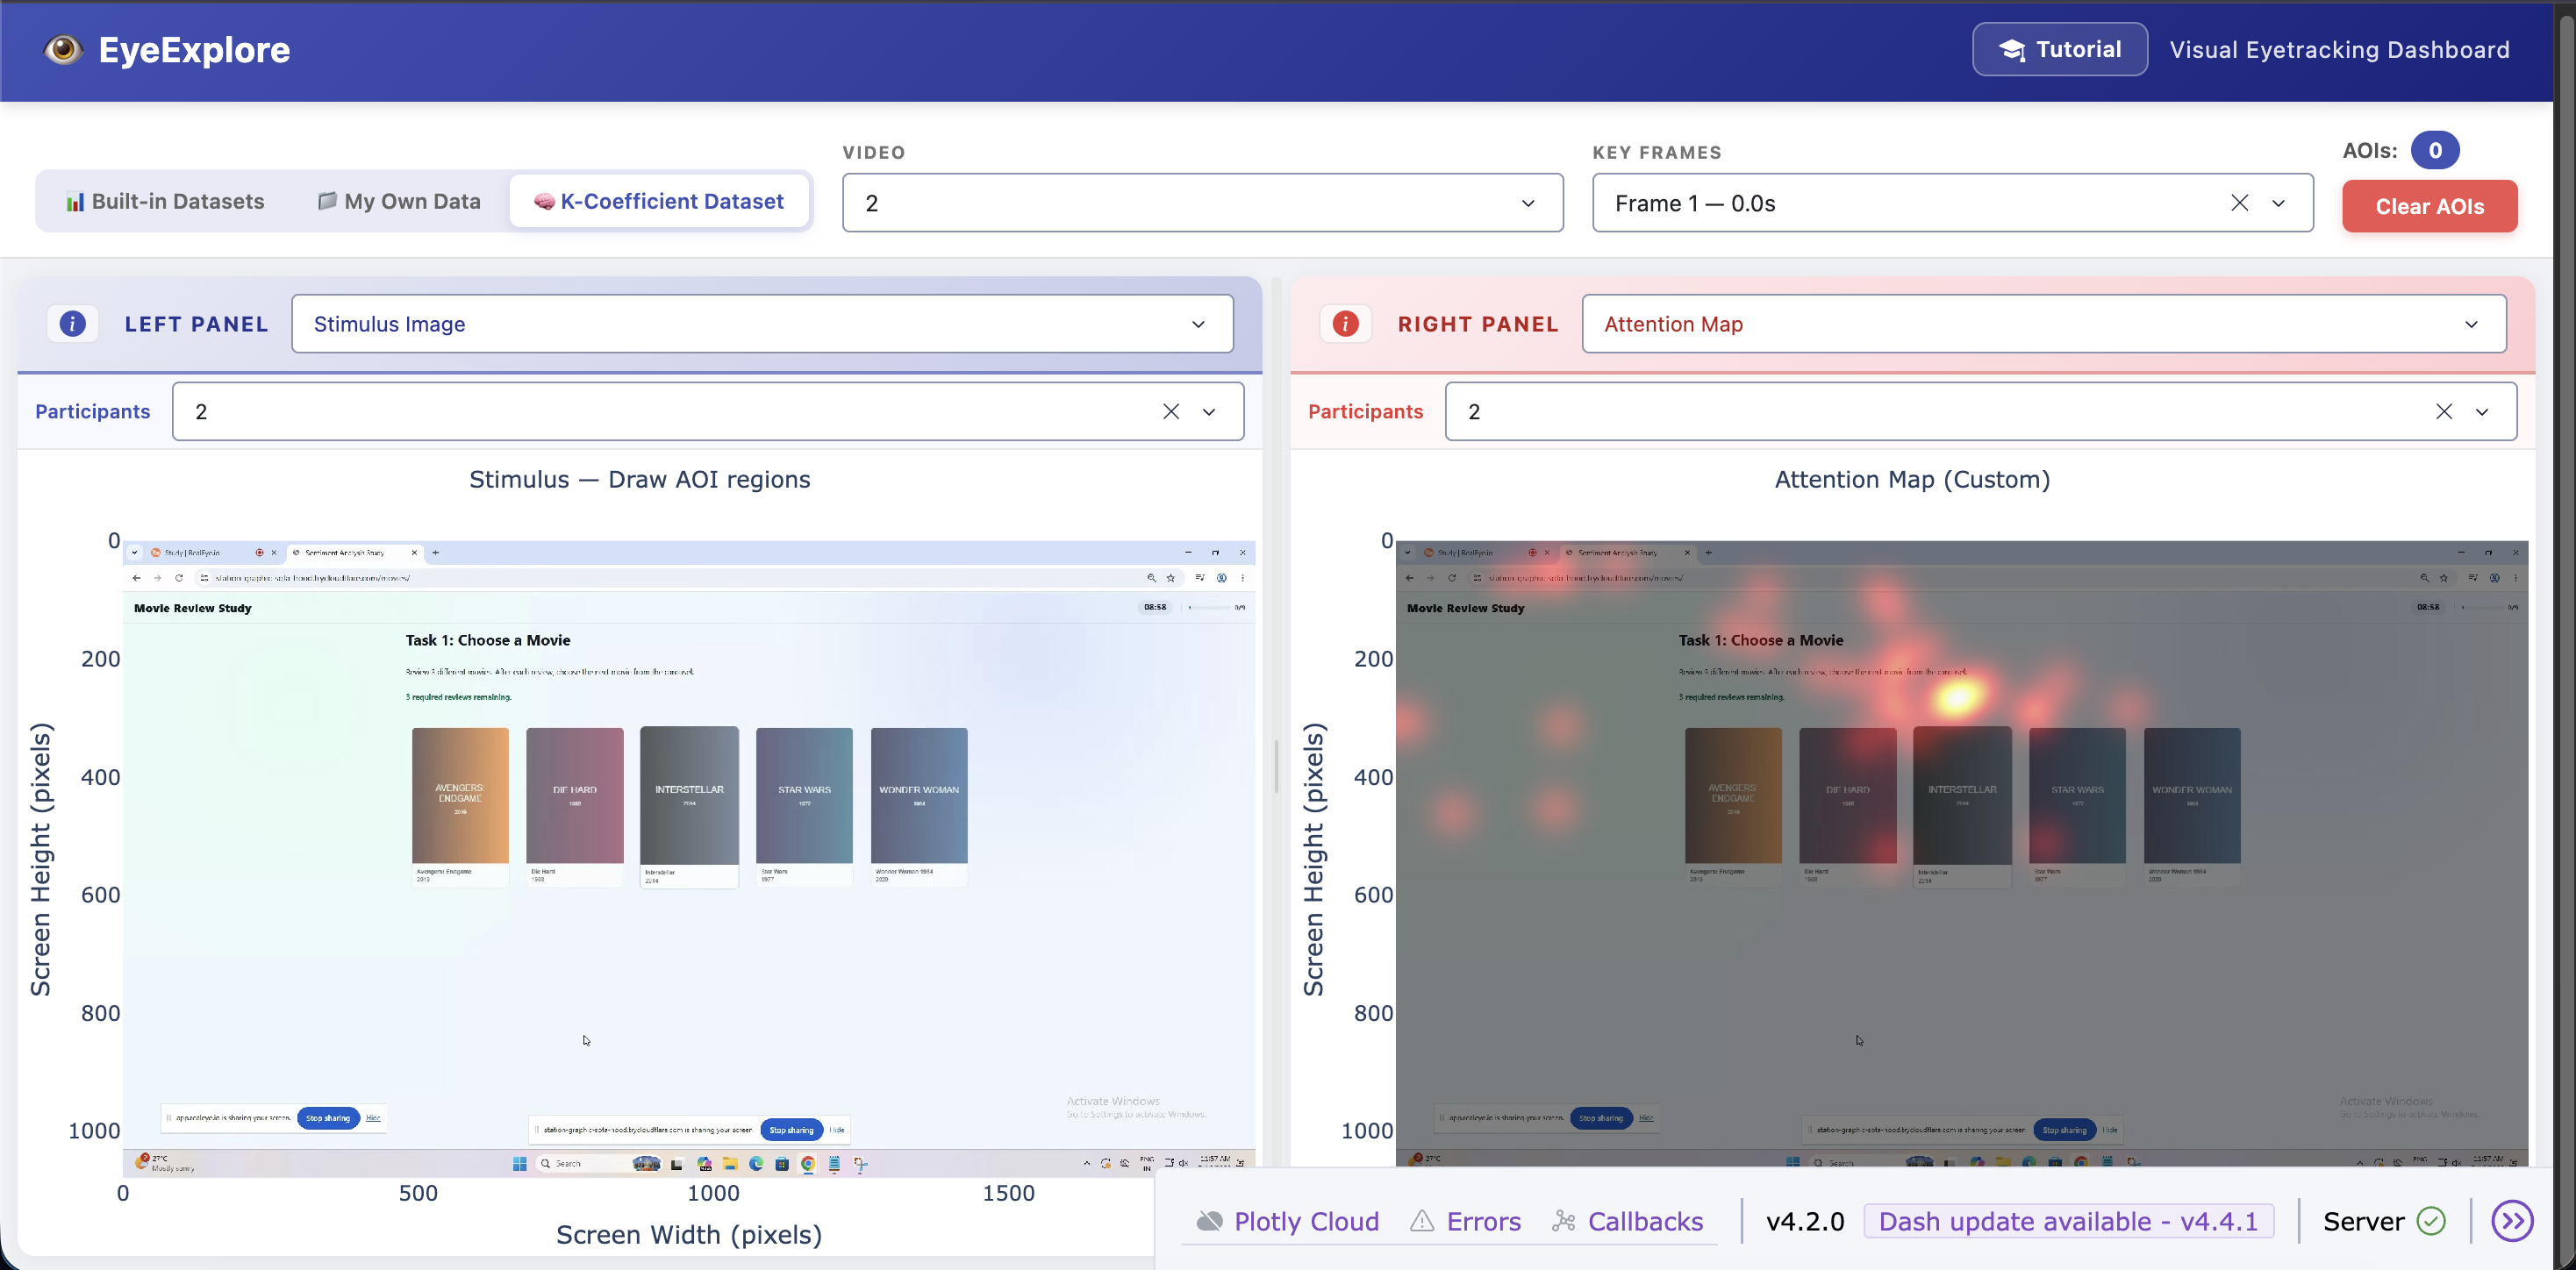
\includegraphics[width=0.98\linewidth]{img3.png}
    \caption{\textbf{"K-Coefficient Dataset" Dashboard Interface:} Displaying video stimulus selection (Video 2), extracted keyframes, and dual-panel comparative visualization (Left: Keyframe with AOI tools, Right: Keyframe Attention Map).}
    \label{fig:k_dataset_dashboard}
\end{figure}

\subsection{Theoretical Foundations of the K-Coefficient}
Human visual exploration oscillates between two distinct cognitive processing modes, first systematically modeled by Unema et al. and Eisenberg \& Zacks:
\begin{enumerate}[noitemsep,topsep=2pt]
    \item \textbf{Ambient Processing Mode:} Characterized by \textit{short fixation durations} followed by \textit{long, exploratory saccades}. The brain rapidly scans the global visual field to identify salient regions of interest.
    \item \textbf{Focal Processing Mode:} Characterized by \textit{long fixation durations} preceded by \textit{short, localized saccades}. Visual attention is deeply concentrated on a specific locus to extract semantic detail (e.g., reading text or inspecting fine features).
\end{enumerate}

To quantify these cognitive transitions, the raw $K$-coefficient ($K_i$) is computed as the normalized difference between fixation duration and preceding saccade amplitude:
\begin{equation}
    K_i = \frac{d_i - \mu_d}{\sigma_d} - \frac{a_i - \mu_a}{\sigma_a}
\end{equation}
where $d_i$ is the duration of fixation $i$, $a_i$ is the amplitude of the preceding saccade, and $\mu_d, \sigma_d, \mu_a, \sigma_a$ denote the mean and sample standard deviation of duration and amplitude across the trial.

To bound extreme outliers while preserving monotonicity and sign, a logistic transformation squashes $K_i$ into the range $[-1, +1]$:
\begin{equation}
    K_{\text{squashed}} = \frac{L}{1 + \exp(-k \cdot K_i)} - 1 \quad \text{with } L = 2, \, k = 0.125
\end{equation}

\subsection{Dataset Scope and Statistical Integrity}
The pre-processed K-Coefficient dataset incorporated into EyeExplore comprises:
\begin{itemize}[noitemsep,topsep=2pt]
    \item \textbf{27 Video Stimuli} (resolutions $1920 \times 1080$, IDs $2$ through $45$).
    \item \textbf{26 Evaluated Participants} with pre-calculated K-metrics.
    \item \textbf{35,350 Total Fixation Events}, of which $34,991$ ($98.98\%$) possess valid computed $K$-values ($1.02\%$ NaN entries occur exclusively at boundary conditions lacking preceding saccade measurements).
    \item \textbf{Statistical Centering:} Across all participants, the aggregate mean $K_{\text{squashed}} = 0.0009 \approx 0$ with $\sigma = 0.105$, confirming rigorous empirical centering around the ambient/focal boundary ($y = 0$).
\end{itemize}

\subsection{Real-Time Video-Timeline Synchronization Architecture (\texttt{k\_sync.js})}
A major engineering challenge was synchronizing dynamic HTML5 video playback with the interactive Plotly timeline chart. Standard Dash server-side callbacks are bounded by network latency ($\sim 100\text{--}300\,\text{ms}$) and cannot sustain 60 FPS animation.

To solve this, a high-performance client-side synchronization engine was written in vanilla JavaScript (\texttt{assets/k\_sync.js}):
\begin{itemize}
    \item \textbf{Decoupled Animation Loop:} Executes an autonomous \texttt{requestAnimationFrame} loop that queries the HTML5 video element's \texttt{currentTime} continuously.
    \item \textbf{Binary Search Lookups ($O(\log N)$):} Fixation events are sorted chronologically. Given \texttt{currentTime}, the closest active fixation is retrieved via binary search, executing in under $0.05\,\text{ms}$.
    \item \textbf{Letterbox Aspect Ratio Projection:} Because the HTML5 video utilizes \texttt{object-fit: contain}, the rendered video surface often differs from the container bounding box due to letterboxing/pillarboxing. The script computes dynamic offsets:
    \begin{align}
        \text{If } \text{AR}_{\text{container}} > \text{AR}_{\text{video}}: & \quad H_{\text{render}} = H_{\text{cont}}, \quad W_{\text{render}} = H_{\text{cont}} \cdot \text{AR}_{\text{video}}, \quad X_{\text{offset}} = \frac{W_{\text{cont}} - W_{\text{render}}}{2} \\
        \text{If } \text{AR}_{\text{container}} \le \text{AR}_{\text{video}}: & \quad W_{\text{render}} = W_{\text{cont}}, \quad H_{\text{render}} = \frac{W_{\text{cont}}}{\text{AR}_{\text{video}}}, \quad Y_{\text{offset}} = \frac{H_{\text{cont}} - H_{\text{render}}}{2}
    \end{align}
    Fixation coordinates are mapped onto pixel space:
    \begin{equation}
        X_{\text{final}} = X_{\text{offset}} + \left(\frac{x_{\text{pct}}}{100}\right) W_{\text{render}}, \quad Y_{\text{final}} = Y_{\text{offset}} + \left(\frac{y_{\text{pct}}}{100}\right) H_{\text{render}}
    \end{equation}
    \item \textbf{Gaze Overlay \& Fading Trail:} Positions a high-contrast black fixation marker (\texttt{\#k-fixation-dot}) and manages an array of trailing history nodes with decaying opacity ($\alpha \in [0.15, 0.70]$) to visualize saccadic path momentum.
    \item \textbf{Throttled Timeline Scrubber Relayout:} Updating Plotly shapes at 60 FPS causes browser thread starvation. The scrubber update is throttled to $100\,\text{ms}$ ($\sim 10$ FPS):
    \begin{lstlisting}[language=Java]
if (Date.now() - lastPlotlyUpdate > 100) {
  Plotly.relayout(plotlyDiv, {
    'shapes[0].x0': currentTime,
    'shapes[0].x1': currentTime
  });
  lastPlotlyUpdate = Date.now();
}
    \end{lstlisting}
    \item \textbf{Resilient DOM Observers:} Uses a \texttt{MutationObserver} to detect when Dash replaces the hidden JSON data container (\texttt{\#k-fixation-data}), automatically rebinding data arrays without requiring full script re-initialization.
    \item \textbf{State Reset on Tab Navigation:} Implements state-clearing hooks in \texttt{app.py} (\texttt{toggle\_mode}) resetting the active graph to \texttt{'stimulus'} when switching away from the K-tab, preventing detached video threads and lingering animation loops.
\end{itemize}

% ==============================================================================
% 7. INTERACTIVE AREA OF INTEREST (AOI) SYSTEM
% ==============================================================================
\section{Interactive Area of Interest (AOI) System}
\label{sec:aoi_system}

Areas of Interest (AOIs) represent the fundamental spatial primitives required for quantitative gaze metrics. The AOI sub-system in EyeExplore was significantly upgraded:
\begin{itemize}[noitemsep,topsep=2pt]
    \item \textbf{Default Rectangle Draw Tool:} The toolbar initialization defaults to the rectangular draw tool, replacing cumbersome freehand lasso tools that produced irregular, hard-to-interpret boundaries.
    \item \textbf{Overlapping AOI Rejection Algorithm:} Overlapping AOIs introduce ambiguity into gaze classification (a single fixation cannot unambiguously belong to multiple mutually exclusive interface elements). An intersection test was implemented in \texttt{app.py}:
    \begin{lstlisting}[language=Python]
def check_aoi_overlap(new_box, existing_boxes):
    for eb in existing_boxes:
        if not (new_box['x1'] < eb['x0'] or new_box['x0'] > eb['x1'] or
                new_box['y1'] < eb['y0'] or new_box['y0'] > eb['y1']):
            return True # Overlap detected -> reject
    return False
    \end{lstlisting}
    If an overlap is detected, the candidate AOI is rejected with a prominent user notification, preserving data validity.
    \item \textbf{Cross-Panel Persistence \& State Synchronization:} Drawn AOIs are maintained in global state stores. Defining an AOI on the Left Panel instantly propagates the region to Scarf Plots, AOI Timelines, or Transition Matrices displayed on the Right Panel.
\end{itemize}

% ==============================================================================
% 8. DOCUMENTATION, QUALITY ASSURANCE, AND EMPIRICAL EVALUATION FRAMEWORK
% ==============================================================================
\section{Documentation, Quality Assurance, and Empirical Evaluation Framework}
\label{sec:documentation_and_evaluation}

In parallel with software development, an exhaustive documentation, quality assurance, and empirical validation suite was created. Located in the \texttt{reports/} directory, these deliverables ensure software reliability, streamline researcher onboarding, and establish a formal methodology for empirical human-subjects evaluations.

\subsection{Comprehensive User Guide Manual}
A 12-page professional manual (\texttt{reports/EyeExplore\_User\_Guide.pdf}) was authored to serve as the definitive onboarding guide for researchers, students, and usability evaluators.
\begin{itemize}[noitemsep,topsep=2pt]
    \item \textbf{Getting Started \& Prerequisites:} Details environment configuration (Python 3.10+, dependency installation) and browser setup across Chrome, Firefox, Safari, and Edge.
    \item \textbf{Detailed Mode Walkthroughs:} Includes annotated screenshots with numbered callout markers for all three modes:
    \begin{itemize}
        \item \textit{Built-in Datasets Mode:} Dataset selection (MIT1003, SIENA12, VisRecall++), stimulus switching, and cohort selection.
        \item \textit{My Own Data Mode:} Step-by-step guidance on uploading static stimuli (PNG, JPG, BMP) or dynamic video clips (MP4, WEBM), format radio selection (4-column explicit vs. 3-column cumulative), column mapping, and 5-row preview verification.
        \item \textit{K-Coefficient Mode:} Video selection across 27 available recordings, keyframe navigation, and participant filtering.
    \end{itemize}
    \item \textbf{Visualization Catalog:} Complete operational breakdown of all 13 visualization types, detailing visual encodings, prerequisite selections, and cognitive interpretations.
    \item \textbf{AOI \& Toolbar Interactions:} Guidelines on drawing non-overlapping rectangle AOIs, clearing regions, and interacting with the Plotly modebar (box zoom, panning, axis resets, and camera PNG downloads).
\end{itemize}

\subsection{Rigorous 63-Test Manual and Interactive Test Runner}
To guarantee enterprise-grade software stability, a comprehensive 19-page testing specification (\texttt{reports/EyeExplore\_Testing\_Manual.pdf}) and an interactive single-page web application (\texttt{EyeExplore\_Test\_Runner.html}) were developed.

\subsubsection{Test Case Distribution}
The testing suite defines \textbf{63 explicit manual test cases} partitioned across 11 functional domains:
\begin{table}[H]
    \centering
    \caption{\textbf{Quality Assurance Test Coverage by Functional Domain}}
    \label{tab:qa_coverage}
    \footnotesize
    \begin{tabularx}{\linewidth}{l c X}
        \toprule
        \textbf{Testing Domain} & \textbf{Cases} & \textbf{Core Verification Scope} \\
        \midrule
        \textbf{Environment Setup (ENV)} & 2 & Clean application boot on port 8050; cross-browser rendering integrity. \\
        \textbf{Built-in Ingestion (BD)} & 5 & Correct population of MIT1003 (1003 stimuli), SIENA12 (12 stimuli), VisRecall++. \\
        \textbf{Built-in Visualizations (VIS)} & 11 & Rendering correctness across all 11 applicable static/animated modalities. \\
        \textbf{Custom Uploads (MOD)} & 13 & Format enforcement, 10MB/50MB size caps, 4-col vs. 3-col mapping, duplicate errors. \\
        \textbf{Custom Analytics (MOD-VIS)} & 8 & Keyframe window filtering, custom video playback, coordinate auto-scaling. \\
        \textbf{K-Coefficient System (KD)} & 10 & Video switching, 60 FPS scrubber sync accuracy, focal/ambient timeline shading. \\
        \textbf{Global \& Navigation (GLOBAL)} & 5 & Tab cycling without stale state, tutorial tour modal, left/right info popups. \\
        \textbf{AOI System (AOI)} & 7 & Rectangle default, overlapping AOI rejection barrier, cross-panel synchronization. \\
        \textbf{Dual-Panel Comparative (DUAL)} & 4 & Independent plot selection, independent participant cohorts, split resize divider. \\
        \textbf{Security \& Edge Cases (SEC)} & 8 & Zero-retention memory checks, path traversal sanitization, empty/malformed CSVs. \\
        \textbf{Performance \& Stress (PERF)} & 4 & Rapid tab switching, 15-participant heatmaps, continuous 2-minute video sync. \\
        \midrule
        \textbf{Total Test Cases} & \textbf{63} & \textbf{Comprehensive manual verification suite} \\
        \bottomrule
    \end{tabularx}
\end{table}

\subsubsection{Interactive Test Runner Application}
In addition to the static PDF manual, an interactive web-based test runner was developed (\texttt{EyeExplore\_Test\_Runner.html}). Built as a standalone, zero-dependency HTML5 application, it allows testers to execute quality assurance protocols in parallel with the dashboard:
\begin{itemize}[noitemsep,topsep=2pt]
    \item \textbf{Dynamic Test State Tracking:} One-click \textit{Pass}, \textit{Fail}, and \textit{Skip} toggles on every test card with instant color-coded visual feedback.
    \item \textbf{Collapsible Step Details:} Cards expand to reveal preconditions, step-by-step procedures, and expected system behavior.
    \item \textbf{Notes \& Defect Logging:} Integrated textareas on every test card allow testers to record defect links, notes, or anomalies.
    \item \textbf{Real-Time Filtering \& Search:} Instant keyword search across test IDs, titles, and tags, complemented by status filter buttons (All, Passed, Failed, Skipped, Untested).
    \item \textbf{Live Session Timer \& Persistence:} Integrated stop-watch tracks cumulative testing duration. All test states, notes, and timers are auto-saved to \texttt{localStorage}, surviving browser reloads.
    \item \textbf{Structured Report Export:} One-click export of complete test runs into standardized CSV spreadsheets or structured JSON audit reports.
\end{itemize}

\subsection{Formal Empirical User Study Hypotheses}
To prepare for peer-reviewed academic validation (targeting venues such as IEEE VIS, ACM CHI, and ACM ETRA), a formal 12-page research specification was drafted (\texttt{reports/EyeExplore\_User\_Study\_Hypotheses.pdf}). It defines \textbf{10 grounded research hypotheses} evaluating the cognitive efficacy, usability, and analytical advantage of EyeExplore:

\begin{table}[H]
    \centering
    \caption{\textbf{Empirical Research Hypotheses for User Study Validation}}
    \label{tab:hypotheses}
    \footnotesize
    \begin{tabularx}{\linewidth}{l p{3.2cm} X l}
        \toprule
        \textbf{\#} & \textbf{Hypothesis Name} & \textbf{Formal Research Proposition} & \textbf{Validated Feature} \\
        \midrule
        \textbf{$H_1$} & Dual-Panel Coordinated Comparison & Users complete comparative gaze analysis tasks with significantly higher accuracy, lower task completion time, and lower cognitive load (NASA-TLX) using the dual-panel layout compared to single-panel tools. & Dual-Panel Architecture \\
        \textbf{$H_2$} & Animated vs. Static Scanpath Analysis & For identifying temporal ordering and revisitation anomalies, Scanpath Animation achieves significantly higher identification accuracy than static overlays, while static overlays excel at spatial distribution tasks. & Scanpath Animation vs. Overlay \\
        \textbf{$H_3$} & Multi-View AOI Pattern Discovery & Augmenting spatial Attention Maps with Scarf Plots and Transition Matrices enables users to identify cross-participant visual strategy divergences that heatmaps alone obscure. & Scarf Plot \& Transition Matrix \\
        \textbf{$H_4$} & Synchronized Video K-Timeline Attribution & Classifying gaze episodes as "ambient search" vs. "focal study" achieves significantly higher agreement with ground truth when using synchronized Video + K-Timeline playback compared to unsynchronized inspection. & Synced Video + K-Timeline \\
        \textbf{$H_5$} & Co-Association Matrix Clustering & Participant similarity clusters derived from the Gaze Co-association Matrix correlate statistically with external task performance cohorts (e.g., successful vs. unsuccessful problem solvers). & Co-Association Matrix \\
        \textbf{$H_6$} & Cross-Representation Triangulation & Free multi-view exploration across complementary representations yields analytical findings that are more reproducible and held with higher analyst confidence than single-view workflows. & Multi-View Triangulation \\
        \textbf{$H_7$} & Progressive Multi-Representation Learning & Structured educational progression from simple (Stimulus $\to$ Heatmap) to complex representations (Scarf $\to$ Transition $\to$ Co-association) builds deeper comprehension than unstructured access. & Visual Scaffolding \\
        \textbf{$H_8$} & Expertise Gap Reduction & Novice analysts using EyeExplore achieve analytical insight quality within $80\%$ of eye-tracking experts within 30 minutes, whereas novices on traditional single-view tools remain significantly below expert levels. & Usability \& Accessibility \\
        \textbf{$H_9$} & YOLO-Assisted Semantic AOIs & AOIs derived via automated YOLOv8 object detection yield significantly higher inter-analyst agreement and semantic coherence compared to subjective manual rectangle drawing. & Automated YOLO AOIs \\
        \textbf{$H_{10}$} & 3D Spatiotemporal Exploration & Tasks requiring identification of temporal revisitations to identical spatial regions achieve significantly higher accuracy in 3D Scanpath/Scatter views than in 2D projections. & 3D Scanpath \& Scatter \\
        \bottomrule
    \end{tabularx}
\end{table}

\subsubsection{Recommended Experimental Protocol}
The study design specifies a within-subjects, Latin Square counterbalanced protocol ($N \ge 24$ analysts for $H_1\text{--}H_4$ and $H_{10}$; $12$ novices $+ 6$ experts for $H_8$; $10$ analyst pairs for $H_9$) powered at $1-\beta = 0.80$ with $\alpha = 0.05$ and expected medium effect size $d = 0.50$.

\subsection{Novice Interview Questionnaire and Cognitive Load Instrument}
To execute the empirical user evaluations, a standardized 4-part assessment instrument was constructed (\texttt{reports/EyeExplore\_Novice\_Interview\_Questionnaire.docx}):
\begin{enumerate}
    \item \textbf{Part 1: NASA-TLX Cognitive Load Assessment:} Evaluates subjective user workload across six validated sub-scales on a continuous 1--21 scale: \textit{Mental Demand}, \textit{Physical Demand}, \textit{Temporal Demand}, \textit{Performance Success}, \textit{Effort Required}, and \textit{Frustration Level}.
    \item \textbf{Part 2: Standardized System Usability Scale (SUS):} Incorporates the industry-standard 10-item Likert scale ($1 = \text{Strongly Disagree}$ to $5 = \text{Strongly Agree}$) to benchmark overall platform usability, learnability, and perceived system complexity.
    \item \textbf{Part 3: Feature-Specific Utility Ratings ($F_1\text{--}F_{10}$):} Targeted 5-point Likert ratings evaluating individual architectural innovations:
    \begin{itemize}[noitemsep,topsep=2pt]
        \item $F_1$: Dual-panel comparison utility for comparative gaze analysis.
        \item $F_2$: Intuitiveness of the interactive AOI drawing tools.
        \item $F_6$: Effectiveness of the K-Coefficient Timeline for distinguishing ambient vs. focal cognitive modes.
        \item $F_8$: Utility of the real-time synchronized video playback and fixation dot overlay.
        \item $F_9$: Clarity and ease of the custom data upload and column mapping workflow.
    \end{itemize}
    \item \textbf{Part 4: Qualitative Interview \& Open-Ended Reflections:} Semi-structured qualitative interview prompts capturing user mental models:
    \begin{itemize}[noitemsep,topsep=2pt]
        \item Ranking top-3 most valuable visualization types vs. most challenging visual representations.
        \item User self-reports on whether visual clutter was experienced and how rapidly gaze insights were synthesized.
        \item Open-ended feedback on interface friction, feature requests, and willingness to adopt EyeExplore for personal research.
    \end{itemize}
\end{enumerate}

% ==============================================================================
% 9. SUMMARY OF ACHIEVEMENTS & MILESTONES
% ==============================================================================
\section{Summary of Achievements and Mid-Term Milestones}
\label{sec:milestones}

Table~\ref{tab:milestones} summarizes the core technical milestones achieved to date:

\begin{table}[H]
    \centering
    \caption{\textbf{Mid-Term Milestone Achievement Matrix}}
    \label{tab:milestones}
    \footnotesize
    \begin{tabularx}{\linewidth}{l X l}
        \toprule
        \textbf{Milestone / Feature} & \textbf{Technical Implementation Scope} & \textbf{Status} \\
        \midrule
        \textbf{Dual-Panel Architecture} & Side-by-side comparison; independent selectors; split divider & \textbf{Completed} \\
        \textbf{Visualization Suite} & 13 total plot types (Scanpath, Scarf, Co-association, YOLO, etc.) & \textbf{Completed} \\
        \textbf{Contextual Info Modals} & Dynamic Bootstrap modals with theoretical \& practical guides & \textbf{Completed} \\
        \textbf{My Own Data Dashboard} & Zero-retention memory upload; multi-format parser; column mapper & \textbf{Completed} \\
        \textbf{Keyframe Algorithm} & Adaptive HSV + grayscale motion thresholding for video slicing & \textbf{Completed} \\
        \textbf{Coordinate Auto-Scaling} & Percentage-to-pixel normalization for high-resolution stimuli & \textbf{Completed} \\
        \textbf{K-Coefficient Analytics} & Ambient/focal z-score modeling; logistic squashing; timeline chart & \textbf{Completed} \\
        \textbf{Video Sync Engine} & Sub-ms binary search; letterbox projection; throttled Plotly scrubber & \textbf{Completed} \\
        \textbf{AOI System Hardening} & Non-overlapping constraint validation; cross-panel synchronization & \textbf{Completed} \\
        \textbf{Quality Assurance Suite} & 63 manual test cases; interactive browser runner; complete test manual & \textbf{Completed} \\
        \bottomrule
    \end{tabularx}
\end{table}

% ==============================================================================
% 10. CONCLUSION & FUTURE WORK
% ==============================================================================
\section{Conclusion and Next Steps}
\label{sec:conclusion}

The development of \textbf{EyeExplore} has successfully achieved all core mid-term deliverables. The system has evolved from a basic single-view visualizer into an enterprise-grade, comparative visual analytics platform. By marrying robust multi-subject spatio-temporal visualizations with cognitive attention modeling (the $K$-coefficient) and a zero-retention custom data ingestion pipeline, EyeExplore provides an indispensable tool for eye-tracking researchers.

\textbf{Planned Objectives for the Final Phase:}
\begin{enumerate}[noitemsep,topsep=2pt]
    \item \textbf{In-Memory Co-Association in Custom Mode:} Refactor the Co-Association Matrix module to compute pairwise similarities entirely from in-memory DataFrames, removing the legacy file-system dependency.
    \item \textbf{Exportable Analytical Reports:} Implement automated PDF/HTML summary exports containing user-selected dual-panel figures, statistical AOI tables, and gaze metrics.
    \item \textbf{Advanced Filtering \& Cognitive Transitions:} Enable filtering of scanpath overlays by cognitive state (e.g., displaying only ambient saccades or only focal fixations on keyframe stimuli).
\end{enumerate}

\vspace{0.5cm}
\begin{center}
    \small \textcolor{gray}{--- End of Mid-Term Progress Report ---}
\end{center}

\end{document}
